\input format.tex

\usepackage{graphicx}
\graphicspath{{cores/}}

\usepackage{environ}
\usepackage{colortbl,array,booktabs}
\usepackage{tabularx}

\colorlet{TablaBordeSuperior}{topcolor}
\colorlet{TablaBordeInferior}{topcolor}
\colorlet{TablaCentroSuperior}{blue!1}
\colorlet{TablaCentroInferior}{blue!20}
\colorlet{FuenteCabeceraTabla}{white}

\newcolumntype{M}[1]{>{\centering\arraybackslash}m{#1}}
%\newcommand{\tabularxcolumn}[1]{>\arraybackslash}m{#1}}

\tcbset{rtab/.style={
freelance,
frame code={
 \path[top color=topcolor,bottom color=topcolor]
   ([yshift=-#1*(\baselineskip+2pt)]interior.north west) --
   ([yshift=-#1*(\baselineskip+2pt)]interior.north east) {[sharp corners]--
    ([yshift=3pt]interior.north east) --
    ([yshift=3pt]interior.north west)} -- cycle;

  },
interior code={},
 }
}

\newcommand\fuentecabecera[1]{\textcolor{black}{\textbf{#1}}}

\begin{document}

\vspace*{3mm}
%% 各章节
\setlength{\arrayrulewidth}{.2pt}
\fontsize{9.3pt}{11pt}\selectfont
\color{gray2}

\begin{center}
\fontsize{16pt}{\baselineskip}\selectfont\color{black70}\bf {二、体重管理方案}
\end{center}

\vspace*{3mm}

\begin{spacing}{1.5}

\indent {\fontsize{9pt}{11pt}\color{black70}\selectfont 根据您目前检测结果,我们专属为您定制了精准减重方案,建议您严格按照方案执行,并在执行方案3个月后
定期复查,助您有效管理体重,保持苗条。}

\vspace*{2mm}

\noindent{\fontsize{11pt}{11pt}\selectfont\color{black70}\bf {微生态减重方案}}

\vspace*{2mm}

\color{black70}\fontsize{9pt}{12pt}\selectfont
\begin{tabular}{m{2.5cm}<{\centering}m{12cm}<{\centering}}
  \parbox[c][0.4cm]{\hsize}{\color{black70}\bf 肠道调理产品} &
  \parbox[c][0.4cm]{\hsize}{\color{black70}\bf 推荐用法用量} \\
      \parbox[c][0.4cm]{\hsize}{\color{black70} 未来优态U2} &
    \parbox[c][0.4cm]{\hsize}{\color{black70} 2次/天,10g/次,午餐及晚餐前十分钟服用效果更佳} \\
      \parbox[c][0.4cm]{\hsize}{\color{black70} 未来优态UA} &
    \parbox[c][0.4cm]{\hsize}{\color{black70} 1次/天,1.5g/次,餐后服用效果更佳} \\
    \multicolumn{2}{l}{\fontsize{8.5pt}{12pt}\selectfont\color{black70} 建议持续服用3-6个月,持续调理肠道菌群,增强肠道菌群对控制体重的作用,帮助减脂减重。}\\
  \multicolumn{2}{l}{\fontsize{8.5pt}{12pt}\selectfont\color{black70} (本方案为推荐方案,具体服用量和服用周期可根据自身实际情况和服用效果进行调整。)}\\
\end{tabular}

\vspace*{3mm}

        \indent\color{black70}\fontsize{8.5pt}{12pt}\selectfont {{\raisebox{1pt}{\color{topcolor}$\divideontimes$}}\! 温馨提示 :益生菌固体饮料为活菌制剂,建议用37℃以下温水冲调并及时服用,以免有益菌失活而影响干预效果}\\
  
\end{spacing}

\vspace*{3mm}

\noindent
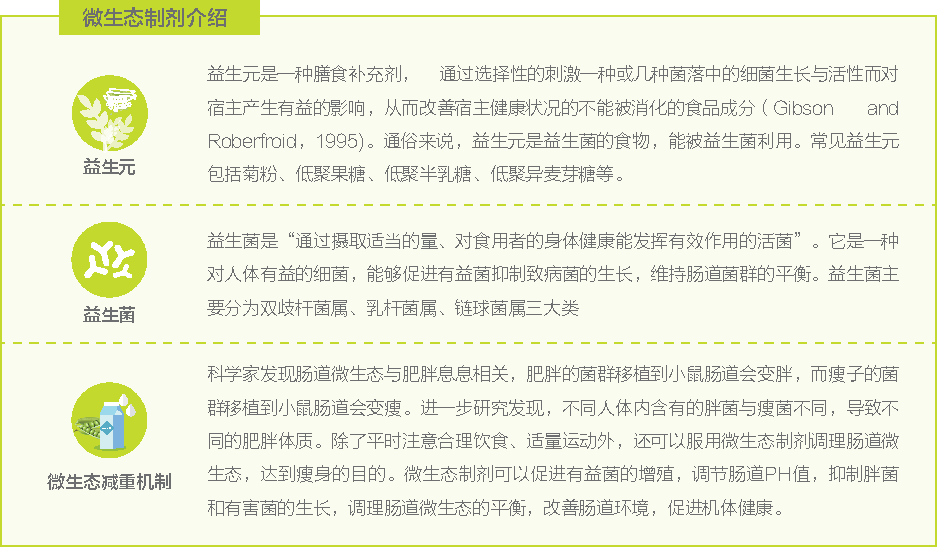
\includegraphics[width=\linewidth]{preprobiotics-intro.pdf}

\end{document}

